\documentclass[english]{article}
\usepackage[T1]{fontenc}
\usepackage[utf8]{inputenc}
%\usepackage{lmodern}
\usepackage[a4paper]{geometry}
\usepackage{babel}
\usepackage{tikz}
\usetikzlibrary{shapes.geometric, arrows}
\usepackage{graphicx}
\usepackage{amsmath}
\usepackage{color}
\usepackage{caption}
\usepackage{subcaption}
\usepackage{amsfonts}
\definecolor{cgreen}{rgb}{0,0.6,0}
\definecolor{cgray}{rgb}{0.5,0.5,0.5}
\definecolor{cpurple}{rgb}{0.58,0,0.82}
\definecolor{darkblue}{rgb}{0.0, 0.0, 0.75}
\definecolor{darkred}{rgb}{0.65, 0.0, 0.0}
\definecolor{darkgreen}{rgb}{0.0, 0.2, 0.13}
\definecolor{cwhite}{rgb}{1,1,1}
\usepackage{listings}
\lstnewenvironment{Python}
{\lstset{language=Python,
		frame=lines, 
		basicstyle=\footnotesize, 	
		commentstyle=\color{darkred},
		keywordstyle=\color{darkblue},
		numberstyle=\tiny\color{cgray},
		stringstyle=\color{cgreen},
		breaklines=true,                 
		numbers=left,
		showtabs=false,                  
		tabsize=2,
		basicstyle=\footnotesize}}{}
\lstnewenvironment{Spark}
{\lstset{language=SQL,
		frame=lines, 
		basicstyle=\footnotesize, 	
		breaklines=true,                 
		showtabs=false,                  
		tabsize=2,
		basicstyle=\footnotesize}}{}\graphicspath{ {./images/} }
\usepackage{a4wide}
\renewcommand{\epsilon}{\varepsilon}

%block for start/stop
\tikzstyle{startstop} = [rectangle, rounded corners, minimum width=3cm, minimum height=1cm,text centered, draw=black, fill=red!30]
%block for input
\tikzstyle{io} = [rectangle, rounded corners, minimum width=3cm, minimum height=1cm, text centered, draw=black, fill=blue!30]
%block for process blocks
\tikzstyle{process} = [rectangle, minimum width=3cm, minimum height=1cm, text centered, draw=black, fill=orange!30]
%block for desicion blocks
\tikzstyle{decision} = [ellipse, minimum width=3cm, minimum height=1cm, text centered, draw=black, fill=green!30]
%arrows
\tikzstyle{arrow} = [thick,->,>=stealth]

\begin{document}
	\begin{titlepage}
		\title{Machine Learning Data Assimilation\\ \vspace{2mm}
			\Large for real time predictions}
		\author{Robin Evers}
		\date{}
		\maketitle
	\end{titlepage}
	{\small\tableofcontents}
\newpage
\section{Introduction}
The aim for this project is to incorporate machine learning algorithms in data assimilation processes in order to improve efficiency and accuracy of numerical simulations. 
We will use observations together with a machine learning (ML) model to perform data assimilation (DA), an uncertainty quantification technique used in order to improve numerical forecasted results. The machine learning model will be created using a time series to emulate the forecasting model. This model together with the observations form the input to the data assimilation process. This results in a forecasting error estimation which we will feed back to the machine learning model as can be seen in Figure \ref{fig:flowchart}. 

This way the assimilation process is trained and we are able to include the obtained information in the ML forecasting model. At each iteration the model learns a function that accumulates the misfit between the results of the forecasting model and the observed data. Finally the model composes the misfit function with the forecasting model and it replaces the forecasting model with the result of the composition. The resulting model includes the features of the DA process and, in this way, the forecasted data are closer to the real observation after each iteration.

\begin{figure}[h]
	\centering
	%nodes used to build the blocks spaced 2cm apart from their centres
	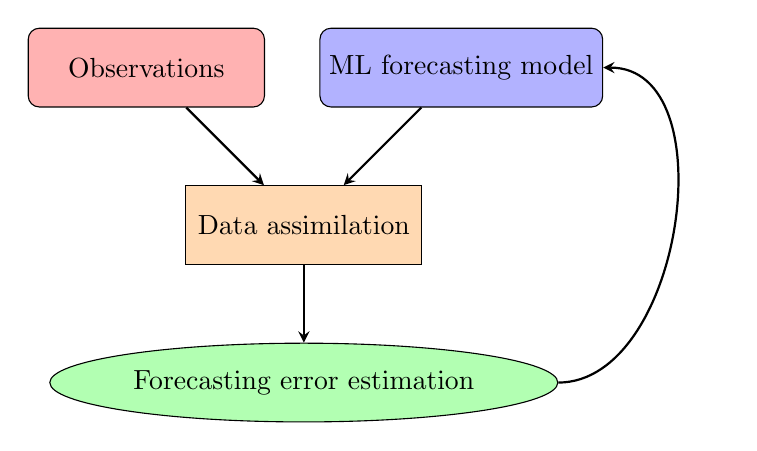
\begin{tikzpicture}[node distance=2cm]
	\node (obs) [startstop] {Observations};
	\node (ML) [io, right of=obs, xshift=2cm] {ML forecasting model};
	\node (DA) [process, below of=obs, xshift=2cm] {Data assimilation};
	\node (error) [decision, below of=DA] {Forecasting error estimation};
	\draw [arrow] (obs) -- (DA);
	\draw [arrow] (ML) -- (DA);
	\draw [arrow] (DA) -- (error);
	\draw [arrow] (error) [out=0, in=0] to (ML);
	\end{tikzpicture} 
	\caption{Schematic view of MLDA model}
	\label{fig:flowchart}
\end{figure}
The machine learning techniques we will describe in section 2 are split up into supervised and unsupervised learning techniques. Under supervised learning we categorise algorithms that use label-containing data. In other words, it observes both the input variables and the corresponding output variables for each datapoint. Unsupervised learning techniques observe only datapoints consisting of input variables, its aim is to find structure in them.

We look at three types of problem, starting with \textit{regression}. This is a supervised learning method in which the labels are continuous values.
Supervised learning techniques for discrete labels are know as \textit{classification}.
Unsupervised learning techniques do not aim to label data, but instead try to find the underlying distribution from which the data might have been generated, this is known as \textit{density estimation}.

We start with regression on linear models, next we look at the discriminative and generative classification approaches. Then we look at dimensionality reduction, clustering and kernel methods. Finally we look at Gaussian process regression and classification. The aim is to look at neural networks and deep learning next. An important part of this report is the implementation and application of the covered machine learning methods to a variety of data sets as this greatly aided the understanding of the uses and limitations of the different methods. In this report the language used is Matlab as it allows for a rapid implementation of algorithm and straightforward visualisation of results.
\vspace{0.5cm}

\noindent The data assimilation techniques used include Kalman filters and variational approaches, these will be discussed in section 3.
\section{Machine learning techniques}
\subsection{Linear regression}
A statistical model consists of two parts, firstly it aims to find the underlying `true' mechanism that generate the observed data and secondly it aims to find an error model capturing the random variability we see. This is often represented as a parametric family of probability distributions. Our first question is, given multiple parametric models, how do we decide which is the most appropriate description? It is important to realise that a mathematical model is only an approximation of reality, hence finding a model that describes the natural systems we observe is not necessarily the best approach. Instead the aim of machine learning is to automatically find the useful models.

The main challenge we face when trying to construct an accurate mathematical model of some natural phenomenon is dealing with the error in our measurements- the variability in the observations. An educated decision has to be taken in determining whether the observed is noise or an important part of the underlying dynamics. 

We generate the following sample data. For $x\in[-5,5]$, define
\begin{equation}\label{firstexample}
	y(x) = 5x^3-x^2+x.
\end{equation}
We interpret $y$ as the phenomenon we want to capture with a model. Let us assume that we can find 100 noisy measurements $y(x)+\epsilon$ where $\epsilon\sim \mathcal{N}(0,100)$. We show the noisy observations in a graph.
\begin{center}
\includegraphics[width=0.5\textwidth]{sampledata.eps}
\end{center}
To analyse the 100 data points using supervised learning, we have to decide upon the choice of functions that we think might be appropriate. 
\subsubsection{The linear parametric model}
Let us first consider a simple linear relationship between $x$ and $y$, writing $\textbf{w}$ for the vector of weight parameters. Our example uses dimension $D=1$, hence $\textbf{x} = (1, x)$ and for the linear relationship we have $\textbf{w}=(w_0,w_1)^T$ 
\begin{equation}\label{linrel}
	h_\textbf{w}(\textbf{x})=w_0+w_1x = \textbf{w}^T\textbf{x}.
\end{equation}
Now that we have chosen a model, we need to learn the parameters $\textbf{w}$. We introduce the loss function $J$ which will measure the mismatch between the measured output and the model output for training pairs $(\textbf{x}^{(i)},y^{(i)})$. By averaging over all $N$ training pairs, this gives the sample average loss function
\begin{equation}
	\frac{1}{N} J \left[y^{(i)}, h_\textbf{w}\left( \textbf{x}^{(i)}\right)\right].
\end{equation}
The loss function is free to be chosen in any way, but a useful example is the sample mean squared error loss
\begin{equation}
\frac{1}{N}  \sum_{i=1}^N \left(y^{(i)} - h_\textbf{w}\left( \textbf{x}^{(i)}\right)\right)^2.
\end{equation}
We write the MSE loss in matrix form by defining 
\begin{align*}
\textbf{w} = \begin{pmatrix}
w_0 \\ w_1
\end{pmatrix} \quad
\textbf{y} = \begin{pmatrix}
y^{(1)} \\ \vdots \\ y^{(N)}
\end{pmatrix} \quad
\textbf{\textbf{X}} = \begin{pmatrix}
1 & {x}^{(1)} \\ \vdots & \vdots \\ 1 & {x}^{(N)}
\end{pmatrix}
\end{align*}
where $\textbf{X}$ is known as the design matrix. This MSE in matrix form now follows as
\begin{equation}
\operatorname{MSE} = \frac{1}{N} (\textbf{y}-\textbf{X}\textbf{w})^T(\textbf{y}-\textbf{X}\textbf{w}).
\end{equation}
To learn the parameters $\textbf{w}$, we minimise the loss function. In this case we can obtain an analytic solution, but for many other problems numerical optimisation is required, we will discuss these later.

For an analytic solution, we take the partial derivative of the MSE function to the parameters $\textbf{w}$ and find its roots. This leads to finding the stationary point
\begin{equation}\label{MSEzero}
\frac{\partial\operatorname{MSE}}{\partial \textbf{w}} = \frac{2}{N} \textbf{X}^T(\textbf{y}-\textbf{X}\textbf{w}) = 0.
\end{equation}
We check that will indeed give a minimum, by checking that the Hessian of the function is positive definite
\begin{equation}
\frac{\partial^2\operatorname{MSE}}{\partial \textbf{w}^2} = \frac{2}{N} \textbf{X}^T\textbf{X},
\end{equation}
which is positive definite when $N>D$.
We solve equation \ref{MSEzero} for $\textbf{w}$ to obtain the least squares estimate 
\begin{equation}\label{wMLE}
\hat{\textbf{w}} = (\textbf{X}^T\textbf{X})^{-1}\textbf{X}^T\textbf{y}.
\end{equation}
Calculating the least squares estimate for our samples from \ref{firstexample} gives
\begin{align*}
\hat{\textbf{w}} = \begin{pmatrix}
-4.6770 \\
\ 80.3705
\end{pmatrix}
\end{align*}
We can use the parameter values we have learned to make predictions at new values in the interval $[-5,5]$, let us denote the design matrix of the new points by $\tilde{\textbf{X}}$, then
\begin{equation}
\hat{\textbf{y}} = \tilde{\textbf{X}} (\textbf{X}^T\textbf{X})^{-1}\textbf{X}^T\textbf{y}.
\end{equation}
\begin{center}
	\includegraphics[width=0.5\textwidth]{sampledatalinearpred.eps}
\end{center}
Lets test how good this model is by testing it against the datapoint $x=10$, we calculate the actual $y$-value corresponding to $x$ using \ref{firstexample} and find that $y=4910$. Using the linear model, we find
\begin{equation}
\hat{y_{10}} = \begin{pmatrix}
1 & 10
\end{pmatrix} \hat{\textbf{w}} = \begin{pmatrix}
1 & 10
\end{pmatrix} \begin{pmatrix}
-4.6770 \\
\ 80.3705
\end{pmatrix} = 799.0281.
\end{equation}
It seems our model predicts values that are too low when $x$ goes up, but too high for decreasing $x$. Using this model to predict $y$ outside the $[-5,5]$ frame is therefore not a good idea.
\subsubsection{Higher order models}
We have seen how to learn parameters for a chosen linear parametric model and mean squared loss function. We tested the model on a cubic generating function and noticed that using it outside the interval on which the training points were defined is not a good idea. Knowing that our observations come from a cubic polynomial, a more complex model based on higher order polynomials will give much more accurate predictions.

An expected cubic relationship between the input variable $\textbf{x}=(1,x)$ and an output variable may be defined by weights $\textbf{w}=(w_0,w_1,w_2,w_3)^T$ as 
\begin{equation}\label{cubicrel}
h_\textbf{w}(\textbf{x})=w_0+w_1x + w_2x^2+w_3x^3 = \textbf{w}^T\textbf{x}.
\end{equation}
or more generally a $k$th order polynomial may be defined by weights $\textbf{w}=(w_0,w_1,\ldots,w_k)^T$ as 
\begin{equation}\label{kpolrel}
h_\textbf{w}(\textbf{x})= \sum_{i=0}^k w_k x^k = \textbf{w}^T\textbf{x}.
\end{equation}
The same derivation for the least squares estimate of $\textbf{w}$ holds if we write the design matrix as
\begin{align*}
\textbf{\textbf{X}} = \begin{pmatrix}
1 & {x^{(1)}}  & {x^{(1)}}^2 & \cdots & {x^{(1)}}^k  \\ \vdots & \vdots & \vdots & \ddots & \vdots \\ 
1 & {x}^{(N)} & {x^{(N)}}^2 & \cdots & {x^{(N)}}^k
\end{pmatrix}.
\end{align*}
We repeat the procedure to find the least squares estimate of $\textbf{w}$ for a 9th order polynomial and plot our findings
\begin{center}
	\includegraphics[width=0.5\textwidth]{sampledata9opred.eps}
\end{center}
The model approximates the 100 datapoints very well, implying a lower empirical loss function. However, we know that the data was generated using a cubic polynomial, hence a lower empirical loss does not always imply a better model.

To determine the predictive power of a parametric model we introduce a technique called cross validation. Cross validation partitions the dataset into 2 disjoint subsets and uses one for training the model and the other for validating the model. We thus learn the parameters $\textbf{w}$ from the training data and then calculate the loss using the validation data. The procedure can be repeated over multiple subsets of the data in which case we can use the average loss as the performance measure. Two possible ways to partition the data are leave-one-out cross validation (LOOCV), where we use the subsets consisting of a single data pair one by one as the validation set, and $K$-fold cross validation, in which we partition the data into $K$ equally sized subsets and use these as the validation sets.
\begin{center}
	\includegraphics[width=0.5\textwidth]{MSE.eps}
\end{center}
As we can see from the plot, cross validation provides an increased measure of performance as it both punishes too simple models and too complex models.

Alternative approaches to prevent overfitting add a regularisation term to the loss function that penalises models with very large parameter values. Examples are ridge regression which employs $\mathcal{L}2$ regularisation and lasso regression, which employs $\mathcal{L}1$ regularisation.
\subsubsection{Probabilistic interpretation}
In the previous sections we used the mean squared error loss function to determine the parameters for a linear model. We will look at the loss function from a probabilistic view now. As in \ref{linrel} we denote the modelled underlying relationship between the input $x$ and output value $y$ by $h_{\textbf{w}}$ where $\textbf{w}$ denotes the weights. We use the error term $\epsilon$ to capture noise and other unmodelled effects, we can choose to model $\epsilon$ however we want, but in this text we will always model noise using a normal distribution.
\begin{equation}
	y = h_{\textbf{w}}(\textbf{x})+\epsilon.
\end{equation}
From here onwards we will accept that observations are made independently of each other and that the noise on the measurements comes from the same distribution $\mathcal{N}(0,\beta^{-1})$ where $\beta$ denotes the precision. In other words, we accept that the data is i.i.d. as an assumption. This assumption allows us to write
\begin{equation}
	p(\textbf{y}|\textbf{X},\textbf{w},\beta) = \prod_{i=1}^{N}p(y^{(i)}|\textbf{x}^{(i)}, \textbf{w}, \beta) = \prod_{i=1}^N\mathcal{N}\left(y^{(i)}|h_\textbf{w}(\textbf{x}^{(i)}), \beta \right)
\end{equation}
This is the likelihood function, maximising it for the parameters $\textbf{w}$ leads to the maximum likelihood solution $\hat{\textbf{w}} = (\textbf{X}^T\textbf{X})^{-1}\textbf{X}^T\textbf{y}$ as in \ref{wMLE}. We can optimise our choice of $\beta$ as well by calculating the stationary point with respect to $\beta$ and finding an analytical solution. Furthermore we can estimate the uncertainty in the parameters $\textbf{w}$ and $\beta$ we inferred by calculating the covariance of the maximum likelihood estimates.
\subsubsection{The Bayesian approach} 
So far we have learned the parameters for our linear models by minimising the loss, or equivalently, by maximising the likelihood $p(\textbf{y}|\textbf{X},\textbf{w},\beta)$. These techniques assumed a `true' underlying set of parameter values and optimised the way to find these. 

We will now look at the Bayesian approach which makes it explicit that we are mostly interested in finding the probability distribution over the parameters, i.e. $p(\textbf{w}, \beta|\textbf{X},\textbf{y})$. But first we will make a small generalisation to the models we consider.

Our previous approach solely considered models that were linear functions of the input variables and the parameters $w_0, \ldots, w_D$ 
\[h_\textbf{w}(\textbf{x})=w_0 +w_1x_1 +...+w_Dx_D \]
where $\textbf{x} = (x_1, \ldots, x_D )^T$. We will now extend this model by considering linear combinations of fixed non-linear functions of the input variables
\begin{equation}\label{linearmodel}
	 h_\textbf{w}(\textbf{x})= \sum_{j=0}^{M-1} w_j \phi_j(\textbf{x}) = \textbf{w}^T \mathbf{\phi}(\textbf{x}).
\end{equation}
where $\phi_j (\textbf{x})$ are known as basis functions, and the weights are given by $\textbf{w} = (w_0,\ldots ,w_{M-1})^T$ and $\mathbf{\phi} = (\phi_0,\ldots ,\phi_{M-1})^T$. We will assume that the $\phi_j(\textbf{x})$ are independent and that $\phi_0(\textbf{x})=1$.
The function $h_\textbf{w}(\textbf{x})$ can now be a non-linear function of the input vector $\textbf{x}$. We call these types of functions linear models, because they are linear in $\textbf{w}$. By keeping the linearity in the parameters, we greatly simplify the analysis of this class of models. Examples of basis functions are polynomials (as considered in the previous sections), Gaussians and sigmoidal functions.

The effective complexity of linear models is governed by the number of basis functions. We need to control this number according to the size of the data set. We can do this by maximising the likelihood when setting the parameters for the model. If we add a regularisation term to the log likelihood function, then the effective model complexity can be controlled by the value of the regularisation coefficient. The choice of the number and form of the basis functions is of course still important in determining the overall behaviour of the model.\newline\newline
\textbf{Parameter distribution}\newline
We start by introducing a prior probability distribution over the model parameters $\textbf{w}$. The likelihood function $p(\textbf{y}|\textbf{w})$ is the exponential of a quadratic function of $\textbf{w}$. The corresponding conjugate prior is therefore given by a Gaussian distribution of the form
\begin{equation}
	p(\textbf{w}) = \mathcal{N} (\textbf{w}|\textbf{m}_0, \textbf{S}_0)
\end{equation}
having mean $\textbf{m}_0$ and covariance $\textbf{S}_0$.

We assume that the target variable $t$ is given by a deterministic function $y(\textbf{x}, \textbf{w})$ with Gaussian noise $\epsilon$
\begin{equation}
y = h_\textbf{w}(\textbf{x}) + \epsilon
\end{equation}  
where $\epsilon$ is a zero mean Gaussian random variable with precision (inverse variance) $\beta$. Therefore we can write
\begin{equation}\label{condtargetvar}
	p({{y}}|\textbf{x}, \textbf{w}, \beta) = \mathcal{N}({{y}}| h_\textbf{w}(\textbf{x)},\beta^{-1}) = \mathcal{N}({{y}}| \textbf{w}^T\phi(\textbf{x}),\beta^{-1}).
\end{equation}
If we write $\Phi$ for the design matrix for the basis functions $\Phi_{nk} = \phi_k(\textbf{x}^{(i)})$ and $\textbf{\textit{t}}$ for the column vector of target variables (predicted output values) $\{y^{(i)}\}$, then 
\begin{equation}
p(\textbf{\textit{t}}|\textbf{x}, \textbf{w}, \beta) = \mathcal{N}({{y}}| \Phi \textbf{w},\beta^{-1}).
\end{equation}
Using the identity for the conditional distribution as in equation (2.116) from Bishop\cite{Bishop}, we find that
\begin{equation}\label{postweightdist}
	p(\textbf{w}|\textbf{\textit{t}}, \textbf{x}, \beta) = \mathcal{N}(\textbf{w}|\textbf{m}_N,\textbf{S}_N)
\end{equation}
where \begin{align}\label{postmean}
\textbf{m}_N &= \textbf{S}_N(\Phi^T\beta\textbf{\textit{t}}+\textbf{S}_0^{-1}\textbf{m}_0) = \textbf{S}_N(\textbf{S}_0^{-1}\textbf{m}_0 + \beta\Phi^T\textbf{\textit{t}}),\\
\textbf{S}_N^{-1} &= \textbf{S}_0^{-1} + \Phi^T\beta\Phi =  \textbf{S}_0^{-1} + \beta\Phi^T\Phi.
\end{align}
We are interested in making predictions for $y$ given new values for $\textbf{x}$, this is the predictive distribution, given by
\begin{equation}\label{preddist}
	p(y|\textbf{\textit{t}}, \textbf{x}, \beta) = \int p(y|\textbf{w}, \textbf{x}, \beta) p(\textbf{w}| \textbf{\textit{t}},\textbf{x},\beta) d\textbf{w}.
\end{equation}
The conditional distribution of the target variable is given by equation \ref{condtargetvar}, and the posterior weight distribution is given by equation \ref{postweightdist}. Since equation \ref{preddist} convolutes two Gaussian distributions, we can use result (2.115) from Bishop\cite{Bishop} to get
\begin{equation}
	p(y|\textbf{\textit{t}},\textbf{x},\beta) = \mathcal{N}(y|\phi(\textbf{x})^T \textbf{m}_N, \beta^{-1}+\phi(\textbf{x})^T \textbf{S}_N\phi(\textbf{x})).
\end{equation}
Note that in the Bayesian approach, we get a posterior distribution over the parameters rather than a single maximum value as in the likelihood approach. By averaging over the posterior distribution we obtained the distribution of our predictions. 
\subsubsection{Equivalent kernel}
If we substitute our equation for the posterior mean \ref{postmean} into the model expression \ref{linearmodel}, we see that the predictive mean can be written as
\begin{align}
	h_{\textbf{m}_N} (\textbf{x}) = \textbf{m}_N^T \phi(\textbf{x}) &= \phi(\textbf{x})^T\textbf{S}_N\textbf{S}_0^{-1}\textbf{m}_0 + \beta \phi(\textbf{x})^T \textbf{S}_N\Phi^T\textbf{\textit{t}} \nonumber \\
	&= \phi(\textbf{x})^T\textbf{S}_N\textbf{S}_0^{-1}\textbf{m}_0 + \sum_{n=1}^N \beta \phi(\textbf{x})^T \textbf{S}_N\phi(\textbf{x}^{(n)}){{y^{(n)}}}.
\end{align}
From this we see that the predictive mean at a point $\textbf{x}$ is a linear combination of the target variables of the training set $\{y^{(n)}\}$, we write
\begin{equation}
	h_{\textbf{m}_N} (\textbf{x})= C(\textbf{x}) + \sum_{n=1}^N k(\textbf{x},\textbf{x}_n)y^{(n)},
\end{equation}
where the equivalent kernel $k$ is given by
\begin{align} \label{kerneldef}
	k(\textbf{x}, \textbf{x}') &= \beta\phi(\textbf{x})^T \textbf{S}_N\phi(\textbf{x}').
\end{align}
We now consider the covariance of $h$ at two time points $\textbf{x}$ and $\textbf{x}'$. Using the equation for the posterior weight distribution \ref{postweightdist} and the definition of the equivalent kernel \ref{kerneldef} we find
\begin{align}
	\operatorname{cov}[h_\textbf{w}(\textbf{x}), h_\textbf{w}(\textbf{x}')] &= \operatorname{cov}[\phi(\textbf{x})^T\textbf{w}, \textbf{w}^T\phi(\textbf{x}')] \nonumber\\
	&= \phi(\textbf{x})^T\textbf{S}_N \phi(\textbf{x}') = \beta^{-1}k(\textbf{x}, \textbf{x}').
\end{align}
This equivalent definition of regression will come in useful when we look at Gaussian processes as it will turn out that Bayesian linear regression is an example of a Gaussian process.
\subsection{Classification}
The contents of this section have been covered in module M5MS10 and include binary and multi-class classification, the discriminative and generative approach and a way of implementing classification methods when analytic solutions are not sufficient (including the Laplace approximation and Newton's method). After this the non-parametric classification approach of $K$-nearest neighbour will be presented 
\subsection{Dimensionality reduction}
Many objects that are of interest in machine learning may be easily described by high dimensional patterns. Images may for example be described by pixel intensity values and documents may be described by word frequencies. Often it is useful to represent such high dimensional objects in lower dimensions as this allows for the compression and visualisation of data and removes dimensions that are not informative.

In this section we will discuss principal component analysis (PCA), which is one of the most common and simple dimensionality reduction techniques. This is an unsupervised model as it does not make any use of labels or outcomes.

Next we will discuss linear discriminant analysis (LDA) which is also a technique for dimensionality reduction. However, unlike PCA, LDA is a supervised method making use of class information. 

Both these techniques have been covered in module M5MS10 and will be added to a later progress report.
\subsection{Density Estimation}
We are often interested in inferring the underlying distribution from which some observed data was generated. An example of this was covered in the generative approach to classification where the class conditional density $p(\textbf{x}|C=k)$ is estimated. This density can be given a parametric form, denoted $p(\textbf{x}|\textbf{w}_k)$ to form a likelihood that can be maximised with respect to the parameters $\textbf{w}$. In this section we shall start with considering parametric approaches to density estimation using maximum likelihood. Next we will consider more complex mixture density models and introduce the EM algorithm for learning the appropriate parameters for this approach.

These techniques have been covered in module M5MS10 and will be added to a later progress report.
\subsection{Cluster analysis}
Cluster analysis allows us to discover subgroups of patterns whose members are more similar to each other than they are to members of other groups. The clusters can provide clear and interpretable meaning in many applications and can be used to label the data, which allows us to train classifiers. 

Cluster analysis is different to dimensionality reduction in the sense that dimensionality would be used to visualise the data and to represent input vectors replacing the original variables, which can then be used to train a classifier on labelled data.

This technique has been covered in module M5MS10 and will be added to a later progress report.
\subsection{Gaussian Processes}
A Gaussian process is a collection of random variables, any finite number of which have a joint Gaussian distribution.  A Gaussian process is completely specified by its mean function and covariance function. We define mean function $m(\textbf{x})$ and the covariance function $k(\textbf{x},\textbf{x}')$ of a real process $f(\textbf{x})$ as
\begin{align}
	m(\textbf{x}) &= \mathbb{E}[f(\textbf{x})], \\
	k(\textbf{x},\textbf{x}') &= \mathbb{E}[(f(\textbf{x})-m(\textbf{x}))(f(\textbf{x}')-m(\textbf{x}'))],
\end{align}
and will write the Gaussian process as 
\begin{equation}
	f(\textbf{x})\sim \mathcal{GP} (m(\textbf{x}),k(\textbf{x},\textbf{x}')).
\end{equation}
The random variables represent the value of the function $f(\textbf{x})$ at location \textbf{x}. For notational convenience we write $f_i$ for the random variable  (RV) corresponding to the case $(\textbf{x}^{(i)},y^{(i)})$.

 An example of a Gaussian process can be obtained from our Bayesian linear regression model $f(\textbf{x}) = \phi(\textbf{x})^T \textbf{w}$ with prior $\textbf{w} \sim \mathcal{N}(0,\Sigma_p)$. We have for the mean and covariance
 \begin{align}
\mathbb{E}[f(\textbf{x})] &= \phi(\textbf{x})^T\mathbb{E}[\textbf{w}]=0, \\
 \mathbb{E}[f(\textbf{x})f(\textbf{x}')] &=\phi(\textbf{x})^T\mathbb{E}[\textbf{w}\textbf{w}^T]\phi(\textbf{x}') =\phi(\textbf{x})^T\Sigma_p\phi(\textbf{x}').
 \end{align}
 Thus $f(\textbf{x})$ and $f(\textbf{x}')$ are jointly Gaussian with zero mean and covariance given by $\phi(\textbf{x})^T\Sigma_p\phi(\textbf{x}')$. Indeed, the function values $f(\textbf{x}_1), \ldots, f(\textbf{x}_n)$ corresponding to any number of input points $n$ are jointly Gaussian, although if $N < n$ then this Gaussian is singular (as the joint covariance matrix will be of rank $N$).
  \begin{figure}[h]
 	\begin{center}
 		\includegraphics[scale=0.45]{priors.eps}
 		\caption{Drawing 5 samples from the GP prior}
 		\label{fig:GPprior}
 	\end{center}
 \end{figure}
 \subsubsection{Squared Exponential Covariance Function}
 In this section we look at the squared exponential (SE) covariance function, defined by
 \begin{equation}\label{covariancesquaredexponential}
\operatorname{cov} \left(f(\textbf{x}_p), f(\textbf{x}_q) \right) = k(\textbf{x}_p, \textbf{x}_q) = \exp  \left( - ||\textbf{x}_p - \textbf{x}_q||^2 \right) .
 \end{equation}
 It can be shown (section 4.3.1,  Rasmussen\cite{Rasmussen}) that the squared exponential covariance function corresponds to a Bayesian linear regression model with an infinite number of basis functions.
 
The kernel is defined only in terms of the spatial separation, therefore it is called a stationary kernel. Such kernels only depend on separation and not the absolute values of $\textbf{x}$, $\textbf{x}'$, which means that wherever in the domain the spatial separation is identical, the covariance will be identical. Additionally, the correlation between inputs decays inversely as a function of distance, i.e., closer inputs are highly correlated as compared to farther inputs.

 The specification of the covariance function implies a distribution over functions. 
 To see this, we can draw samples from the distribution of functions evaluated at any number of points; in detail, we choose a number of input points, $X_*$ and write out the corresponding covariance matrix using equation (\ref{covariancesquaredexponential}) element wise. 
Then we generate a random Gaussian vector with this covariance matrix
\begin{equation}
	f_* \sim \mathcal{N} (0,K(X_*,X_*))
\end{equation}
and plot the generated values as a function of the inputs. Figure \ref{fig:GPprior} shows samples from a GP prior that are generated like this using 100 input points uniformly distributed between $-\frac12$ and $2\pi + \frac12$. 
\begin{figure}[h]
	\begin{center}
		\includegraphics[scale=0.45]{posteriors.eps}
		\caption{Drawing 5 samples from the GP posterior}
		\label{GPposterior}
	\end{center}
\end{figure}
\newline\newline
\textbf{Prediction with Noise-free Observations}
\newline
We are usually not primarily interested in drawing random functions from the prior, but want to incorporate the knowledge that the training data $X$ provides about the function. Initially, we will consider the simple special case where the observations are noise free, that is we know $\{(\textbf{x}_i , f_i ) | i = 1, \ldots , n\}$. 
The joint distribution of the training outputs $f$ and the test outputs $f_*$ according to the prior is
\begin{align}
	\begin{pmatrix}
	\textbf{f} \\
	\textbf{f}_*
	\end{pmatrix}
	\sim \mathcal{N} \left( \textbf{0},
	\begin{pmatrix}
	K(X,X) & K(X,X_*) \\
	K(X,X_*)^T & K(X_*, X_*)
	\end{pmatrix}
	\right).
\end{align}
Here we wrote $K(X,X)$ to represent the auto-correlation between the inputs $X$ and $K(X,X_*)$ represents the cross-correlations between the observed and unobserved inputs. Similarly, $K(X_*,X_*)$ represents auto-correlation amongst the unobserved inputs $X_*$ . Shorthand for all the aforementioned kernels are $K, K^*, K^{**}$ in the respective order.

To get the posterior distribution over functions we need to restrict this joint prior distribution to contain only those functions that agree with the observed data points. In probabilistic terms this operation corresponds to conditioning the joint Gaussian prior distribution on the observations to give
\begin{equation}\label{31}
	p(\textbf{f}_*|X_*, X, \textbf{f}) \sim \mathcal{N}(\boldsymbol{\mu}_{f|D}, K_{f|D}),
\end{equation}
where we write $D=[X,Y]$ for the training dataset. The posterior mean and covariance are given by
\begin{equation}
	\boldsymbol{\mu}_{f|D} = K(X_*,X)K(X,X)^{-1}\textbf{f} = {K^*}^T K^{-1} \textbf{f}.
\end{equation}
This equation can be seen a linear estimator with $\boldsymbol{\mu}_{f|D} = {K^*}^T \boldsymbol{\alpha}$ for $\boldsymbol{\alpha} = K^{-1}\textbf{f}$ and this in fact, is the best linear unbiased estimator.
\begin{equation}
	K_{f|D} = K(X_*, X_*) - K(X_*, X)K(X, X)^{-1}K(X, X_*) = K^{**}-{K^*}^TK^{-1}K^*.
\end{equation}
Notice that ${K^*}^TK^{-1}K^*$ can be interpreted as the evidence, showing that the variance reduces as more evidence is acquired from observations.

\begin{figure}[h]
	\centering
%	\begin{minipage}{.45\textwidth}
		\begin{minipage}[c]{.45\linewidth}
			\centering
			\includegraphics[width=\linewidth]{posteriorsunscaled.eps}
			\caption{Fitting the original GP to the scaled data}
			\label{GPscaled}
		\end{minipage}
%	\end{minipage}
\hfil
%	\begin{minipage}{.45\textwidth}
		\begin{minipage}[c]{.45\linewidth}
			\centering
			\includegraphics[width=\linewidth]{posteriorsscaled.eps}
			\caption{Fitting the scaled GP to the scaled data}
			\label{GPfitted}
		\end{minipage}
%	\end{minipage}
\end{figure}
Function values $f_*$ (corresponding to test inputs $X_*$) can be sampled from the joint posterior distribution by evaluating the mean and covariance matrix from equation \ref{31}. To demonstrate this we define the underlying distribution on $X$ as a sine, we consider the case where the observations are given by $\{(x^{(i)},\sin(x^{(i)}))|i=1,\ldots 8\}$ where the values of the training inputs $X$ are uniformly 8 distributed points between $0$ and $2\pi$. The results are plotted in Figure \ref{GPposterior}.

The confidence bound (the grey filled area) looks acceptable and we are satisfied with the data fit of the posterior GP. We have however been fortunate with our choice of underlying observation as we have not yet encountered the amplitude of the signal $\sigma_{sig}$. The signal variance indicates the factor by which the kernel function should be scaled to obtain the right distribution. To visualise this we see what happens when we scale the data by a constant factor. We use inputs $\{(x^{(i)},5\sin(x^{(i)}))|i=1,\ldots 8\}$ where the values of the training inputs $X$ are again 8 uniformly distributed points between $0$ and $2\pi$. Figure \ref{GPscaled} shows the result of samples drawn from the GP posterior if we do not scale the kernel function. 

\noindent Using the Maximum Likelihood Estimation (MLE), we try to infer the data scale $\tau = 2\sigma_{sig}$ that fits the data best. We use the optimal signal variance $\sigma_{sig}^2$ to compute the predictive variance again. This gives us the samples drawn from the scaled GP posterior in Figure \ref{GPfitted}.
\newline\newline
\textbf{Predictions with noisy observations}
\newline
This section will explain how the method from section 7.1.1 should be altered in order to be used on noisy data. We will again use MLE methods to determine the hyperparameter for the noise $\sigma_{n}$.
\newpage
\section{Neural Networks}
The study of artificial neural networks is inspired by the knowledge of the biological nervous system and in particular by its centre; the brain. The main components of the nervous system are called neurons, which are electrically excitable cells. Neurons are the cells that function as information processing devices and operate by using the set of fibers that emanate from the cell body. The axon, which is one of these fibers, is responsible for transmitting information to other neurons. The remaining fibers are called dendrites, they are responsible for the propagation of information that is received from other neurons to the cell body. According to many estimates, the human brain contains around 100 billion neurons that are highly interconnected, making the brain an extremely complicated system. Making a true model of the brain would therefore be exceptionally difficult. However, by using simplified models this task becomes feasible and leads us to the study of artificial neural networks.

Artificial neural networks are computational models that use densely interconnected and adaptive processing units that we can think of as neurons. A network consists of a big number of relatively simple processors that work on these units to model a system. We assume that a complex relationship exists between the input to and output from the network. Since the processors can work in parallel, a neural network can be use to replace a classical method to find the corresponding output to a given input and has the potential to significantly speed up the process.

Let us take a closer look at the artificial neurons. The artificial neurons form the elementary units in an artificial neural network, they receive one or more inputs $x_1, x_2, \ldots$ representing the information that is propagated from other neurons by the neural dendrites. An artificial neuron sums these inputs, usually separately weighted with weights $w_i$, and passes the sum through a non-linear function $\varphi$. This function is known as the activation function. Figure \ref{fig:neuron} gives a schematic representation of this process.

\begin{figure}[h]
	\centering
	%nodes used to build the blocks spaced 2cm apart from their centres
	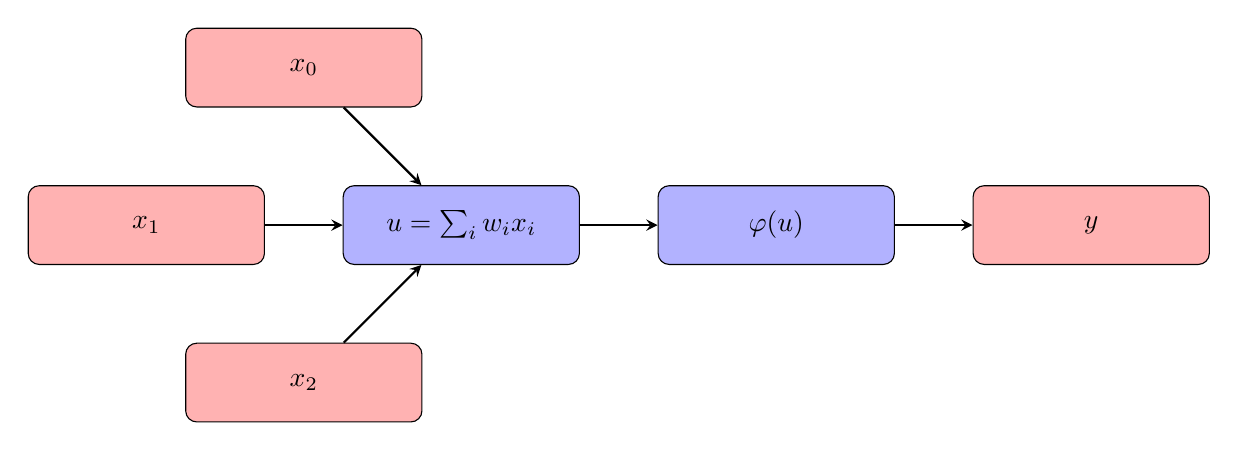
\begin{tikzpicture}[node distance=2cm]
	\node (u) [io] {$u = \sum_i w_i x_i$};
	\node (x1) [startstop, left of=u, xshift=-2cm] {$x_1$};
	\node (x0) [startstop, above of=x1, xshift=2cm] {$x_0$};
	\node (x2) [startstop, below of=x1, xshift=2cm] {$x_2$};
	\node (phi) [io, right of=u, xshift=2cm] {$\varphi(u)$};
	\node (y) [startstop, right of=phi, xshift=2cm] {$y$};
	\draw [arrow] (x0) -- (u);	
	\draw [arrow] (x1) -- (u);	
	\draw [arrow] (x2) -- (u);
	\draw [arrow] (u) -- (phi);
	\draw [arrow] (phi) -- (y);
	\end{tikzpicture} 
	\caption{Schematic view of an artificial neuron}
	\label{fig:neuron}
\end{figure}

The red boxes represent observed valuables. Purple boxes represent values computed as a function of one or more arguments. Finally, the arrows indicate that the source of the arrow is an argument of the function computed at the destination of the arrow.

Each artificial neuron is constituted by one or more inputs - in the example above there were two inputs, $x_1$ and $x_2$ - and one output $y$. Outputs for one neuron can function as inputs of other neurons. In the  summation, the inputs are multiplied by weights $w_i$ and are summed with one constant $x_0$. Finally this sum $v$ goes through the activation function $\varphi$. The activation function works to activate or inhibit the next neuron and can be of several types. The most commons types include the identity function, step functions and sigmoid functions.

We now give a mathematical description of the $k$'th neuron
\[u_k = \sum_{i=1}^n w_{ki} x_i \text{ and } y_k = \varphi(u_k - w_{k0}).\]
Here the inputs are given by $x_0, \ldots x_n$ and the weights are given by $w_{k1},\ldots, w_{kn}$. The weighted sum is denoted by $u_k$. We denote the bias of the $k$'th neuron by $w_{k0}$, its activation function by $\varphi$ and its output by $y_k$.

Neural networks consist of multiple layers. We call the first layer of an artificial neural network the input layer and the last layer the output layer. We will refer to the intermediary layers as the hidden layers.  The number of layers and the quantity of neurons in the layers is flexible and therefore determined by the application.

\subsection{Feedforward Neural Networks}
When using a layered neural network, we organise the neurons in layers. The input layer consists of source nodes and projects onto an output layer of neurons. When the neurons do not project back onto the previous layer, we speak of a feedforward network. When we add hidden layers to our network, we call the resulting network a multilayer feedforward network. The inputs to the neurons in each of the layers in this network come from the outputs of the preceding layer only. A schematic view is given in figure .. This type of architecture suffices for most statistical applications.
\subsection{Recurrent Neural Networks}
If our network contains at least one neuron that connects with one neuron of the preceding layer, a feedback loop is created in the network. We call this type of network a recurrent neural network. This is the type of architecture that is commonly used in optimization problems. A schematic view of a recurrent neural network is given in figure ..

\subsection{Neural Network for Lorenz63}
We use a long short-term memory (LSTM) network to forecast time series data for the Lorenz63 system. To forecast the values of future time steps of the system, we train a sequence-to-sequence regression LSTM network. Because we aim to predict the new time steps from the previous, the response sequence equals the training sequence with values shifted by one time step. The LSTM network will therefore learn to predict the value of the next time step at each time step of the input.

To forecast the values of multiple time steps in the future, we use the \texttt{predictAndUpdateState} function in matlab to predict time steps one at a time and update the network state at each prediction. We train the LSTM network to forecast the $x$, $y$ and $z$ coordinates of the system given the coordinates of the previous time step.

\section{Data assimilation}
This section will cover the Kalman filter and variational approaches to data assimilation. I have started reading on the subject, using section 5 from the book by Kalnay \cite{Kalnay} as my main resource. Other resources that I am planning to use to gain a deeper understanding on this topic include \cite{Asch} and \cite{DARC}.

Data assimilation (DA) methodologies incorporate observational data into prediction models to improve the confidence levels in computational predictions (i.e. improve numerical forecasted results).
Let us observe a forecasting model
\begin{equation}\label{forecasting_model}
	\dot{u} = \mathcal{M}(u,t,\theta)
\end{equation}
where $u$ is a function denoting the state of the model at time $t\in[0,T]$, $\mathcal{M}$ is a non-linear map and $\theta$ is a model parameter.
An observation $v$ of the state $u$ is given by
\begin{equation}\label{observation}
	v = \mathcal{H}(u)+\epsilon_M
\end{equation}
where $\mathcal{H}$ is an observation function and $\epsilon_M$ denotes the measurement error.

Since we will be using computer simulations, we consider discretised versions of the above equations. We can choose the time steps $\Delta t$ small enough to approximate linearly:
\begin{equation}
u_t + \Delta u \approx M(u_t) + M'\Delta u.
\end{equation}
Here $u_k$ denotes the estimated state of the system at time $k$, $M:u_{k}\mapsto u_{k+\Delta t}$ is the discretisation of a first order approximation of $\mathcal{M}$ and $M'$ is the matrix obtained by the first order approximation of the Jacobian of $\mathcal{M}$.
Similarly, for the observation function:
\begin{equation}
\mathcal{H}(u_t +\Delta u) \approx H(u_t) + H'\Delta u.
\end{equation}
We let $v_k$ denote the observation of the system at time $k$, so that $H:u_k\mapsto v_k$ is the discretisation of a first order approximation of $\mathcal{H}$ and $H'$ is the matrix obtained by the first order approximation of the Jacobian of $\mathcal{H}$.

DA aims to `obtain the best possible knowledge of the system as a function of time' and to estimate $\theta$ by using observations $v_k$ and the forecasting model as in \ref{forecasting_model}.
In other words, DA finds a function $u^{DA}$ that is true to the observations (i.e. $u^{DA}$ is likely to have been the actual state of the system given observations $v_k$)
\begin{equation}
 v_k = Hu^{DA} + \epsilon_{R_k},
\end{equation}
but is also true to the model (i.e. $u^{DA}$ is likely to have been the actual state of the system given estimated system states $u_k$)
\begin{equation}
u^{DA}=u_k+\epsilon_{B_k}.
\end{equation}
In the above equations, we incorporated the observation error $\epsilon_{R_k}$, which contains the measurement error $\epsilon_M$, and the model error $\epsilon_{B_k}$. 

We look further into these error terms. Let $E()$ represent the expected value and let us denote the bias of the measurement by $\mu_R$ and the bias of the model error by $\mu_B$, the biases are given by
\begin{equation}
	E(v_k-Hu^{DA}) = \mu_R, \quad E(u^{DA}-u_k)=\mu_B.
\end{equation}
Equivalently we can write
\begin{equation}
	E(\epsilon_{R_k})=\mu_R, \quad E(\epsilon_{B_k})=\mu_B.
\end{equation}
Now that we know the mean of the error terms, we look into their covariance matrices. Starting with the measurement error, we know the variance of the observational error for each observation $k$
\begin{equation}
	E((\epsilon_{R_k}-\mu_R)^2) = E(\epsilon_{R_k}^2)-\mu_R^2 = \sigma_0^2.
\end{equation} 
Hence the observation covariance matrix is given by 
\begin{equation}
	\textbf{R} := E(\epsilon_{R_k}\epsilon_{R_k}^T) =  \sigma_0^2 I.
\end{equation}
The forecast or background error covariance matrix is advanced using the model itself, rather than estimating it as a constant covariance matrix. We know that $\textbf{B}= \epsilon_{B}^{n+1}(\epsilon_{B}^{n+1})^T$, therefore we want to derive an expression for $\epsilon^{n+1}_B$ in terms of $n$'th time step error terms.


We can now write the error terms as Gaussian distributions, for the observation error we have $\epsilon_{R_k}\sim \mathcal{N}(\mu_R, R_k)$, and for the model error $\epsilon_{B_k}\sim \mathcal{N}(\mu_B, B_k)$. 


%Using Bayes' theorem we find that
%\begin{equation}
%u^{DA} = 
%\end{equation}
%We see that $u^{DA}$ maximises 'a probability density function' given the observation $v$ and a prior $u$. Therefore $u^{DA}$ includes information from both the forecasting model and the observation.


\newpage
\section{Experiments}
In this section we apply the DDA technology to the Lorenz system. In 1963 Lorenz developed a simplified mathematical model for atmospheric convection. It is a popular test case for DA algorithms. The model is a system of three ordinary differential equations (the Lorenz equations). It is notable for having a chaotic behaviour for certain parameter values and initial conditions. The Lorenz equations are given by the non-linear system:
\begin{align} \label{lorenz_x}
	\frac{dx}{dt} &= - \sigma(x-y)\\ \label{lorenz_y}
	\frac{dy}{dt} &= \rho x - y - xz\\\label{lorenz_z}
	\frac{dz}{dt} &= xy -\beta z
\end{align}
where $x = x(t)$, $y = y(t)$, $z = z(t)$ and $\sigma,\rho,\beta$ are parameters, which in these experiments are chosen to have the values 10, 28 and 8/3 respectively. We show how the state of the dynamical system (the three variables of a three-dimensional system) evolve over time in a complex, non-repeating pattern.
\begin{figure}[h]
	\centering
	\includegraphics[width=0.5\linewidth]{lorenz.eps}
	\caption{The Lorenz attractor for parameter values $\rho=10, \sigma=28, \beta=8/3$.}
\end{figure}

This Lorenz system can be discretized by second order Runge-Kutta method as in [19]. This gives the following discrete equations:
\begin{align}\label{discrete_lorenz_x}
	x^{k+1} &= x^k + \frac{\sigma\Delta t}{2} \left( 2(y^k - x^k) + \Delta t(\rho x^k - y^k - x^kz^k) -\sigma \Delta t(y^k - x^k)\right) \\ \nonumber \label{discrete_lorenz_y}
	y^{k+1} &= y^k + \frac{\Delta t}{2} \big(\rho x^k - y^k - x^kz^k + \rho(x^k + \sigma\Delta t(y^k -x^k))-y^k \\ &\quad - \Delta t (\rho x^k -y^k -x^kz^k) - (x^k + \sigma\Delta t(y^k - x^k))(z^k + \Delta t(x^ky^k - \beta z_k))\big)   \\ \nonumber \label{discrete_lorenz_z}
	z^{k+1} &= z^k + \frac{\Delta t}{2} \big( x^ky^k -\beta z^k + (x^k + \Delta t \sigma(y^k-x^k))(y^k+\Delta t (\rho x^k - y^k - x^kz^k)) \\
	&\quad -\beta z^k -\Delta t (x^ky^k - \beta z^k)\big).
\end{align}
Here $\Delta t$ is the model time step and $k$ is the time step index. 

We denote the state of the Lorenz system at timestamp $k$ as $u^k = (x^k, y^k, z^k)^T$ and the discrete function as in equations \ref{discrete_lorenz_x}, \ref{discrete_lorenz_y}, \ref{discrete_lorenz_z} as $M^k(\cdot)$. We define a Lorenz system with structural model uncertainty as
\begin{equation}
	u^k = M^k(u^{k-1}) + \xi_{smu,k}
\end{equation}
in which the structural model uncertainty is $\xi_{smu,k} = c u^{k-1}$ (in this case $c = 0.01$).

To compare the accuracy of the DDA technology we first find the true value $u$ by running the system as defined in equations \ref{lorenz_x}, \ref{lorenz_y}, \ref{lorenz_z} using the chosen parameter values. Next we generate what we will use as the observation by adding Gaussian noise on to $u$, we will denote the observation by $v$. 

We are now ready to run the DDA process on the observation. First we apply the DA algorithm to $v$ to obtain $v_{DA}$. We find the discretisation of $v_{DA}$ to create the training set $\{M^k(v^{k-1}_{DA}),v^k_{DA}\}$. This training set is now used to train the neural network $\mathcal{G}_w$.
\section{Plans for the project at this point}
The aim for this project is to incorporate machine learning algorithms in data assimilation processes in order to improve efficiency and accuracy of numerical simulations. The obvious next step is therefore to continue studying and gain a deeper understanding of mathematical, numerical and algorithmic approaches to data assimilation. The next subjects to cover specifically are the Kalman filter and 3D variational approach.

Additionally a further understanding of machine learning algorithms will be developed, specifically on recurrent neural networks.

After this stage, the aim is to develop and apply Machine Learning Data Assimilation (MLDA) algorithms combining Variational approaches, Kalman filter methods and Recurrent Neural Network (RNN) approaches to the processing of the states of forecasting models to improve speed, efficiency and accuracy. 

Firstly a machine learning model will be created using a time series to emulate the forecasting model. Then RNN will be used to train the assimilation process and include this information into the machine learning forecasting model. 

During the MRes phase, synthetic data produced by dynamical systems will be used, such as the double integral mass dot system and the Lorenz system. The main objective after gaining theoretical knowledge is therefore the design of an accurate and efficient model for Machine Learning with Data Assimilation for synthetic data produced by a dynamical system, e.g. the double integral mass dot system or the Lorenz system.

The final goal is to implement the numerical and algorithmic approaches and their validation on computing architectures.

Books used so far include Barber\cite{Barber}, Bishop\cite{Bishop},  Murphy\cite{Murphy}, Rasmussen\cite{Rasmussen} and the Matrix Cookbook\cite{Matrix}.
\bibliographystyle{plain}
\bibliography{bibliography}
\end{document}